\documentclass[aspectratio=169]{beamer}

% ============================================================
% THEME & COLORS
% ============================================================
\usetheme{metropolis}
\usepackage[utf8]{inputenc}
\usepackage{graphicx}
\usepackage{booktabs}
\usepackage{amsmath}
\usepackage{tikz}
\usetikzlibrary{positioning, shapes.geometric}
\usepackage{xcolor}
\usepackage{colortbl}
\usepackage{hyperref}
\hypersetup{colorlinks=true, urlcolor=skyblue, linkcolor=avblue, citecolor=avblue}

% Aviation color palette
\definecolor{avblue}{RGB}{0, 48, 107}       % Deep navy
\definecolor{skyblue}{RGB}{0, 119, 190}     % Sky blue
\definecolor{lightsky}{RGB}{224, 240, 252}  % Light blue background
\definecolor{safegreen}{RGB}{39, 174, 96}   % Success green
\definecolor{alertred}{RGB}{192, 57, 43}    % Warning red
\definecolor{warnorange}{RGB}{230, 126, 34} % Caution orange
\definecolor{lightgray}{RGB}{248, 249, 250} % Slide background

% Apply colors
\setbeamercolor{normal text}{fg=avblue}
\setbeamercolor{frametitle}{bg=avblue, fg=white}
\setbeamercolor{progress bar}{fg=skyblue, bg=lightsky}
\setbeamercolor{title separator}{fg=skyblue}
\setbeamercolor{alerted text}{fg=skyblue}
\setbeamercolor{block title}{bg=avblue, fg=white}
\setbeamercolor{block body}{bg=lightsky, fg=avblue}
\setbeamercolor{block title alerted}{bg=alertred, fg=white}
\setbeamercolor{block body alerted}{bg=lightgray, fg=avblue}
\setbeamercolor{block title example}{bg=safegreen, fg=white}
\setbeamercolor{block body example}{bg=lightgray, fg=avblue}

% Typography
\metroset{progressbar=frametitle, sectionpage=progressbar, block=fill}
\setbeamerfont{title}{size=\Large, series=\bfseries}
\setbeamerfont{frametitle}{size=\normalsize, series=\bfseries}

% ============================================================
% TITLE INFO
% ============================================================
\title{Aircraft Predictive Maintenance}
\subtitle{Machine Learning for Proactive Component Failure Detection}
\author{Jean Plaubert RUKUNDO}
\institute{Civil Aviation Project}
\date{2026}

% ============================================================
\begin{document}
% ============================================================

% ----------------------------------------------------------
% TITLE SLIDE
% ----------------------------------------------------------
\begin{frame}
\titlepage
\end{frame}

% ----------------------------------------------------------
% AGENDA
% ----------------------------------------------------------
\begin{frame}{Agenda}
  \setbeamertemplate{section in toc}[sections numbered]
  \tableofcontents[hideallsubsections]
\end{frame}

% ============================================================
\section{Problem \& Motivation}
% ============================================================

\begin{frame}{Why Predictive Maintenance?}

  \begin{columns}[T]
    \begin{column}{0.48\textwidth}
      \begin{alertblock}{Current Reality}
        \begin{itemize}
          \item Maintenance teams react \textbf{after} failures
          \item No early warning system in place
          \item Failures occur unexpectedly mid-operation
        \end{itemize}
      \end{alertblock}
    \end{column}
    \begin{column}{0.48\textwidth}
      \begin{block}{Business Impact}
        \begin{itemize}
          \item Unplanned maintenance costs \textbf{30--40\% more}
          \item Flight delays \& aircraft downtime
          \item Critical safety risks if failures go undetected
        \end{itemize}
      \end{block}
    \end{column}
  \end{columns}

  \vspace{0.6cm}

  \begin{exampleblock}{Our Goal}
    \centering
    Predict component failures \textbf{before they happen} using real-time sensor data
  \end{exampleblock}

\end{frame}

% ============================================================
\section{Data \& Methodology}
% ============================================================

\begin{frame}{Dataset Overview}

  \begin{columns}[T]
    \begin{column}{0.42\textwidth}
      \textbf{Dataset}
      \begin{itemize}
        \item \textbf{6,000} maintenance records
        \item 12 sensor features per record
        \item Binary target: sensor drift flag (failure indicator)
      \end{itemize}

      \vspace{0.3cm}

      \textbf{Sensor Inputs}
      \begin{itemize}
        \item Temperature sensors 1 \& 2
        \item Vibration \& pressure sensors
        \item Flight cycles \& engine hours
        \item Fault code counts
      \end{itemize}

      \vspace{0.3cm}

      \begin{exampleblock}{Key Insight}
        \small Failing components show \textbf{distinct sensor signatures} before failure
      \end{exampleblock}
    \end{column}

    \begin{column}{0.55\textwidth}
      \textbf{Class Imbalance --- Before \& After SMOTE}

      \vspace{0.3cm}

      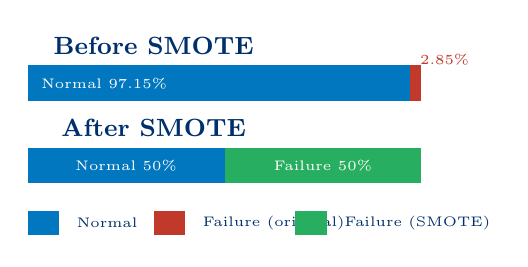
\begin{tikzpicture}
        % ---- BEFORE SMOTE ----
        \node[font=\small\bfseries, text=avblue] at (1.6, 3.6) {Before SMOTE};

        % Normal bar (97%)
        \fill[skyblue]   (0, 2.9) rectangle (4.85, 3.35);
        \fill[alertred]  (4.85, 2.9) rectangle (5.0, 3.35);
        \node[font=\tiny, text=white, anchor=west] at (0.05, 3.12) {Normal 97.15\%};
        \node[font=\tiny, text=alertred, anchor=west] at (4.86, 3.42) {2.85\%};

        % ---- AFTER SMOTE ----
        \node[font=\small\bfseries, text=avblue] at (1.6, 2.55) {After SMOTE};

        % Balanced bars (50/50)
        \fill[skyblue]  (0, 1.85) rectangle (2.5, 2.3);
        \fill[safegreen](2.5, 1.85) rectangle (5.0, 2.3);
        \node[font=\tiny, text=white, anchor=center] at (1.25, 2.075) {Normal 50\%};
        \node[font=\tiny, text=white, anchor=center] at (3.75, 2.075) {Failure 50\%};

        % ---- LEGEND ----
        \fill[skyblue]   (0,   1.2) rectangle (0.4, 1.5);
        \node[font=\tiny, text=avblue, anchor=west] at (0.5, 1.35) {Normal};
        \fill[alertred]  (1.6, 1.2) rectangle (2.0, 1.5);
        \node[font=\tiny, text=avblue, anchor=west] at (2.1, 1.35) {Failure (original)};
        \fill[safegreen] (3.4, 1.2) rectangle (3.8, 1.5);
        \node[font=\tiny, text=avblue, anchor=west] at (3.9, 1.35) {Failure (SMOTE)};
      \end{tikzpicture}

      \vspace{0.1cm}
      \begin{alertblock}{}
        \small \textbf{34:1 imbalance} --- a naive model just predicts ``always normal'' and misses every failure
      \end{alertblock}
    \end{column}
  \end{columns}

\end{frame}

\begin{frame}{Preprocessing Pipeline}

  \begin{center}
  \begin{tikzpicture}
    \tikzstyle{step} = [rectangle, rounded corners,
      text width=2.0cm, minimum height=1.0cm, text centered,
      draw=avblue, fill=lightsky,
      font=\scriptsize\bfseries, text=avblue]
    \tikzstyle{arrow} = [thick, ->, >=stealth, color=skyblue]

    \node (clean) [step]                         {\textbf{1}\\ Clean Data};
    \node (scale) [step, right=0.35cm of clean]  {\textbf{2}\\ Scale Features};
    \node (smote) [step, right=0.35cm of scale]  {\textbf{3}\\ SMOTE Balance};
    \node (split) [step, right=0.35cm of smote]  {\textbf{4}\\ Train/Test Split};
    \node (train) [step, right=0.35cm of split]  {\textbf{5}\\ Train Model};

    \draw [arrow] (clean) -- (scale);
    \draw [arrow] (scale) -- (smote);
    \draw [arrow] (smote) -- (split);
    \draw [arrow] (split) -- (train);
  \end{tikzpicture}
  \end{center}

  \vspace{0.4cm}

  \begin{columns}[T]
    \begin{column}{0.24\textwidth}
      \begin{block}{1 — Clean}
        Remove duplicates; \textbf{keep outliers} --- they signal failures
      \end{block}
    \end{column}
    \begin{column}{0.24\textwidth}
      \begin{block}{2 — Scale}
        StandardScaler: $x' = \frac{x-\mu}{\sigma}$ so no sensor dominates
      \end{block}
    \end{column}
    \begin{column}{0.24\textwidth}
      \begin{block}{3 — SMOTE}
        Synthetic oversampling: balances data to 50/50 failure ratio
      \end{block}
    \end{column}
    \begin{column}{0.24\textwidth}
      \begin{block}{4/5 — Split \& Train}
        80\% train (balanced), 20\% test (stratified split)
      \end{block}
    \end{column}
  \end{columns}

\end{frame}

\begin{frame}{Why Logistic Regression?}

  \begin{columns}[T]
    \begin{column}{0.60\textwidth}
      \textbf{3 Models Trained \& Compared}

      \vspace{0.3cm}
      \begin{tabular}{lcccc}
        \toprule
        \textbf{Model} & \textbf{Recall} & \textbf{Precision} & \textbf{ROC-AUC} & \textbf{Chosen?} \\
        \midrule
        Logistic Regression & \textcolor{safegreen}{\textbf{100\%}} & 52.3\% & 98.76\% & \textcolor{safegreen}{\textbf{Yes}} \\
        Random Forest       & 52.9\%                                & 51.4\% & 98.47\% & \textcolor{alertred}{No} \\
        XGBoost             & 64.7\%                                & 50.0\% & 98.52\% & \textcolor{alertred}{No} \\
        \bottomrule
      \end{tabular}
    \end{column}

    \begin{column}{0.37\textwidth}
      \begin{exampleblock}{Why It Won}
        \begin{itemize}
          \item \textbf{100\% recall} --- only model to catch every failure
          \item Interpretable for maintenance teams
          \item Fast real-time predictions
          \item Outputs probability scores
        \end{itemize}
      \end{exampleblock}
    \end{column}
  \end{columns}

\end{frame}

% ============================================================
\section{Model Performance}
% ============================================================

\begin{frame}{Results at a Glance}

  \begin{columns}[T]
    \begin{column}{0.48\textwidth}
      \begin{center}
        \begin{tabular}{lc}
          \toprule
          \textbf{Metric} & \textbf{Score} \\
          \midrule
          Accuracy  & 97.42\% \\
          Recall    & \textcolor{safegreen}{\textbf{100\%}} \\
          Precision & 52.3\% \\
          ROC-AUC   & \textcolor{safegreen}{\textbf{98.76\%}} \\
          \bottomrule
        \end{tabular}
      \end{center}

      \vspace{0.3cm}

      \begin{exampleblock}{\textcolor{safegreen}{Recall = 100\%}}
        Every real failure caught. \textbf{Zero undetected failures.}
      \end{exampleblock}

      \vspace{0.2cm}

      \begin{block}{Precision = 52.3\%}
        47.7\% false alarms --- triggers \textbf{preventive} checks, not emergencies.
      \end{block}
    \end{column}

    \begin{column}{0.48\textwidth}
      
\includegraphics[width=\textwidth]{confusion_matrix.png}
    \end{column}
  \end{columns}

\end{frame}

\begin{frame}{Evaluation Curves}
  \begin{center}
    
\includegraphics[width=0.85\textwidth]{evaluation_curves.png}
  \end{center}
\end{frame}

\begin{frame}{Threshold Optimization}
  \begin{columns}[T]
    \begin{column}{0.55\textwidth}
      
\includegraphics[width=\textwidth]{threshold_optimization.png}
    \end{column}
    \begin{column}{0.42\textwidth}
      \begin{block}{What This Shows}
        \begin{itemize}
          \item Default threshold = 0.5
          \item We tuned threshold to maximize \textbf{recall}
          \item Safety priority: catching every failure outweighs false alarms
        \end{itemize}
      \end{block}
      \vspace{0.3cm}
      \begin{exampleblock}{Result}
        Threshold set to achieve \textbf{100\% recall} while keeping precision acceptable
      \end{exampleblock}
    \end{column}
  \end{columns}
\end{frame}

% ============================================================
\section{Explainability \& Reliability}
% ============================================================

\begin{frame}{Explainable Predictions with SHAP}

  \begin{columns}[T]
    \begin{column}{0.55\textwidth}
      
\includegraphics[width=\textwidth]{shap_explainability.png}
    \end{column}

    \begin{column}{0.42\textwidth}
      \textbf{How to Read This}
      \begin{itemize}
        \item Each bar = one sensor's contribution
        \item \textcolor{alertred}{Red} = pushes toward failure
        \item \textcolor{skyblue}{Blue} = pushes toward normal
        \item Longer bar = stronger influence
      \end{itemize}

      \vspace{0.3cm}

      \begin{alertblock}{Why It Matters}
        Maintenance teams know \textit{exactly which sensors} triggered an alert --- enabling targeted inspections instead of full checks
      \end{alertblock}
    \end{column}
  \end{columns}

\end{frame}

\begin{frame}{Long-Term Reliability: Data Drift Monitoring}

  \begin{columns}[T]
    \begin{column}{0.55\textwidth}
      
\includegraphics[width=\textwidth]{data_drift_monitoring.png}
    \end{column}

    \begin{column}{0.42\textwidth}
      \begin{alertblock}{The Risk}
        Sensor distributions shift over time --- the model degrades silently without monitoring
      \end{alertblock}

      \vspace{0.3cm}

      \textbf{Monitoring Schedule}
      \begin{itemize}
        \item \textbf{Weekly:} KS drift test on all sensors
        \item \textbf{Monthly:} Recall \& accuracy check
        \item \textbf{Quarterly:} Retrain if needed
      \end{itemize}

      \vspace{0.3cm}

      \begin{exampleblock}{Auto Response}
        Drift detected $\rightarrow$ retrain.\\
        Recall $< 95\%$ $\rightarrow$ fallback to rule-based system.
      \end{exampleblock}
    \end{column}
  \end{columns}

\end{frame}

% ============================================================
\section{Live Deployment}
% ============================================================

\begin{frame}{System Architecture}

  \begin{columns}[T]
    \begin{column}{0.50\textwidth}
      \textbf{Technology Stack}

      \vspace{0.3cm}
      \begin{tabular}{ll}
        \toprule
        \textbf{Layer} & \textbf{Technology} \\
        \midrule
        Frontend  & React.js \\
        Backend   & FastAPI (Python) \\
        ML Model  & Logistic Regression \\
        Cloud     & Railway.app \\
        \bottomrule
      \end{tabular}

      \vspace{0.4cm}

      \textbf{API Endpoints}
      \begin{itemize}
        \item \texttt{POST /predict} --- Single prediction
        \item \texttt{POST /predict\_batch} --- Batch predictions
        \item \texttt{GET /model\_info} --- Model metrics
        \item \texttt{GET /docs} --- Interactive docs
      \end{itemize}
    \end{column}

    \begin{column}{0.46\textwidth}
      \begin{exampleblock}{Live URL}
        \small\href{https://civil-aviationprojectaircraftmaintenance-production.up.railway.app}{\texttt{civil-aviationprojectaircraftmaintenance-\\production.up.railway.app}}
      \end{exampleblock}

      \vspace{0.3cm}

      \textbf{Maintenance Team Workflow}
      \begin{enumerate}
        \item Sensor data submitted to API
        \item Model returns risk score \& label
        \item High-risk alert triggers inspection
        \item Component replaced \textbf{before} failure
      \end{enumerate}
    \end{column}
  \end{columns}

\end{frame}

% ============================================================
\section{Conclusion}
% ============================================================

\begin{frame}{What Was Delivered}

  \begin{columns}[T]
    \begin{column}{0.48\textwidth}
      \begin{exampleblock}{Technical Deliverables}
        \begin{itemize}
          \item[\textcolor{safegreen}{\checkmark}] 100\% recall --- zero failures missed
          \item[\textcolor{safegreen}{\checkmark}] 98.76\% ROC-AUC
          \item[\textcolor{safegreen}{\checkmark}] SHAP explainability
          \item[\textcolor{safegreen}{\checkmark}] Drift monitoring \& retraining plan
          \item[\textcolor{safegreen}{\checkmark}] Live 24/7 REST API
          \item[\textcolor{safegreen}{\checkmark}] Full web interface
        \end{itemize}
      \end{exampleblock}
    \end{column}

    \begin{column}{0.48\textwidth}
      \begin{block}{Business Outcomes}
        \begin{itemize}
          \item \textbf{Safety:} No undetected failures
          \item \textbf{Cost:} Planned vs.\ emergency maintenance
          \item \textbf{Trust:} Explainable AI decisions
          \item \textbf{Longevity:} Self-monitored quality
        \end{itemize}
      \end{block}

      \vspace{0.3cm}

      \begin{alertblock}{Next Steps}
        \begin{itemize}
          \item Integrate with scheduling system
          \item Extend to more component types
          \item Explore time-series deep learning
        \end{itemize}
      \end{alertblock}
    \end{column}
  \end{columns}

\end{frame}

% ----------------------------------------------------------
% CLOSING SLIDE
% ----------------------------------------------------------
\begin{frame}[standout]
  \centering
  \Large\textbf{Thank You}

  \vspace{0.8cm}
  \normalsize

  \textbf{Live Application}\\
  \small\href{https://civil-aviationprojectaircraftmaintenance-production.up.railway.app}{\texttt{civil-aviationprojectaircraftmaintenance-production.up.railway.app}}

  \vspace{0.5cm}
  \normalsize
  \textbf{Interactive API Docs}\\
  \small\href{https://civil-aviationprojectaircraftmaintenance-production.up.railway.app/docs}{\texttt{.../docs}}

  \vspace{0.8cm}
  \normalsize
  Questions welcome.
\end{frame}

\end{document}
